
With a rest mass that is 200 times greater than that of the electron,
muons deposit a small fraction of their energy in the calorimeter. The
muon spectrometer system, positioned just outside of the calorimeters, precisely
measures the muon momentum in the range $|\eta| < 2.7$ to complement
the measurement provided by the ID~\cite{bib:Aad:2008zzm}. It also triggers on muons in
$|\eta|<2.4$. This system has been designed to measure muon momenta up
to $O(1 \tev)$ with a relative resolution of 10\%. In order to
do so, there are three layers of precision tracking chambers; in the
barrel, these layers are concentric cylinders at ($R=5$, 7.5, 10~m),
and in each end-cap the chambers form four parallel disks in the $x$-$y$
plane at $z=7.4$, 10.8, 14.0, 21.5~m. Superconducting toroidal magnets
provide a B-field for the precision measurement. Fast trigger chambers
are capable of providing rough muon track information in 10s of
nanoseconds, allowing a trigger decision to be made. The high temporal
resolution of these chambers makes it possible to match a muon to the
associated beam crossing. Figure~\ref{chap:detector:fig:muon_system}
shows the geometry of the muon system. 

\begin{figure}[ht]
    \centering
    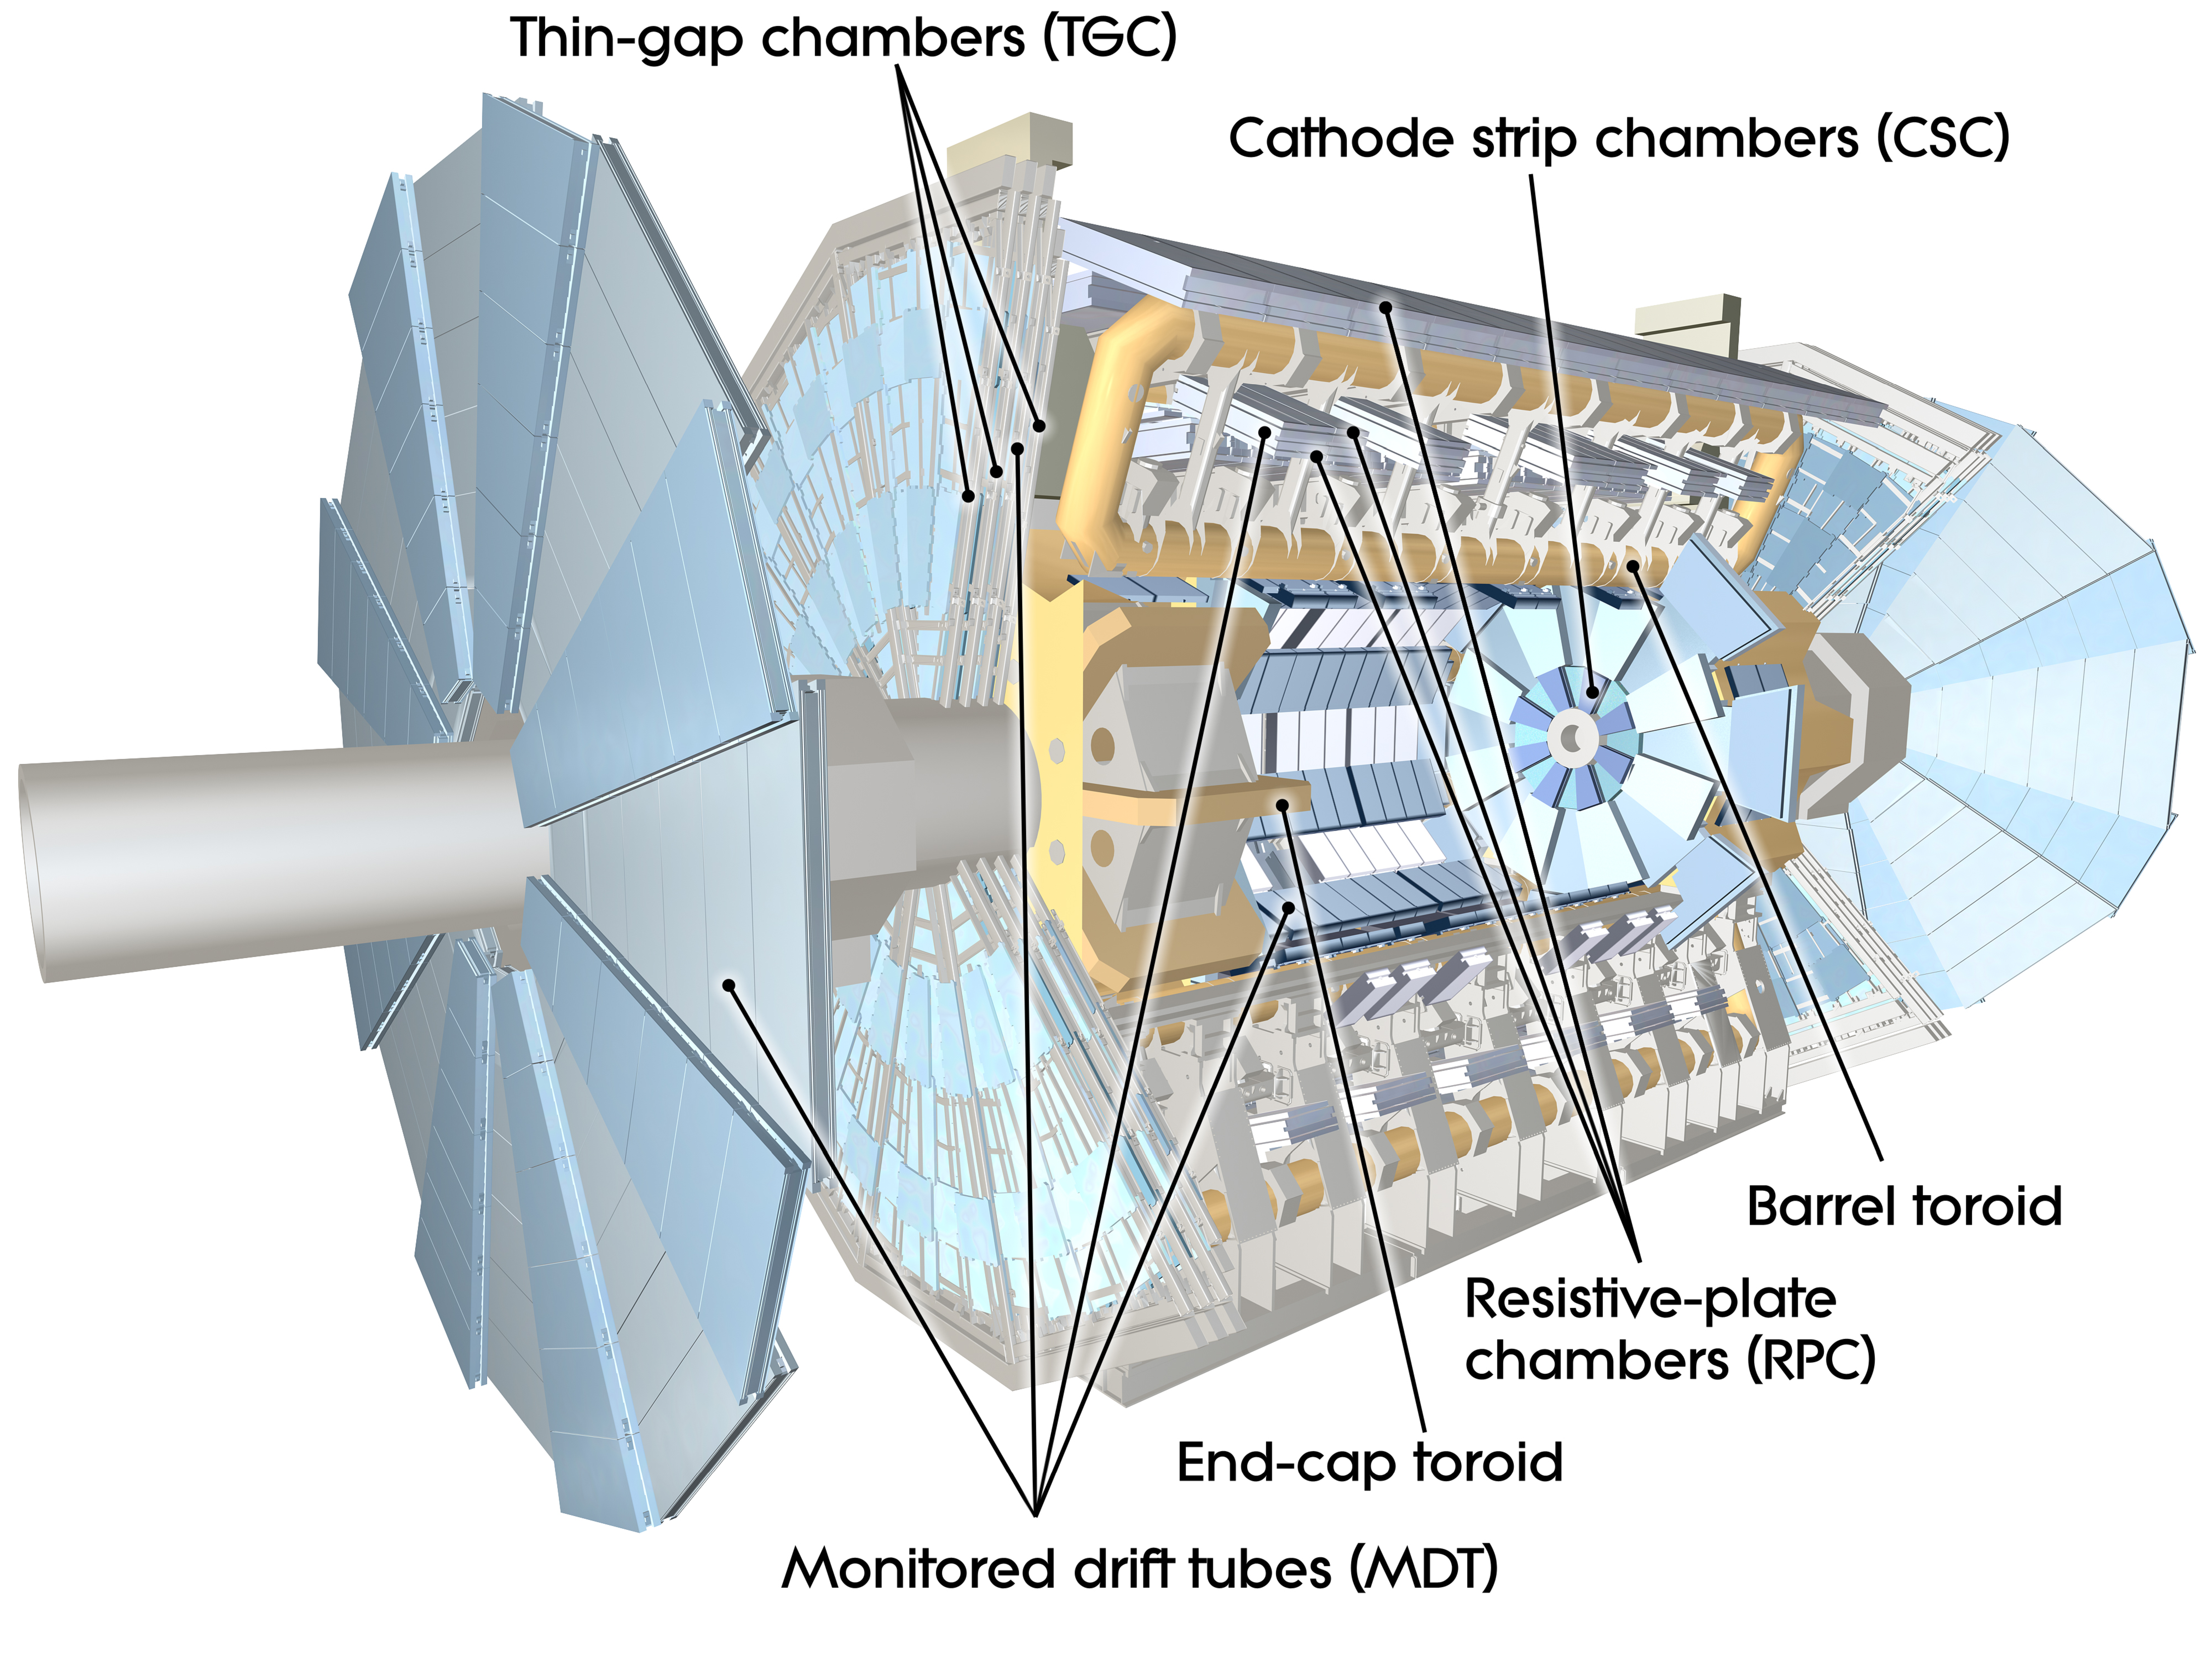
\includegraphics[width=0.8\textwidth]{fig/detector/muon_system.pdf}
    \caption[]{}
\label{chap:detector:fig:muon_system}
\end{figure}

\subsection{High precision tracking chambers}

The precision tracking system consists of three (four) layers of
chambers in the barrel (end-cap) that are immersed in a toroidal
magnetic field. In the barrel, there are eight toroidal magnetic coils
positioned symmetrically in $\phi$, and for each coil, there is a pair
of chambers. The chamber pairs form an alternating set of large and
small rectangular chambers, with adjacent chambers overlapping in $\phi$ to
minimize acceptance loss. In the end-caps, each wheel is also composed
of overlapping large and small chambers, but the geometry of the
chambers is trapezoidal. 

Two precision tracking technologies have been adopted. The predominant
chamber type is the monitored drift tube chamber (MDT). These chambers
contain parallel 3.0~cm copper tubes that run parallel to the $\phi$
direction in both the barrel and end-caps. Inside of the tube is a 50
\micron tungsten-rhenium wire at 3080~V that collects the ionization
electrons from interactions between incident muons and the ArCO$_2$
gas between the tube and the anode. Tubes are arranged into layers and
segmented in $\eta$ and $\phi$. Parallel tubes are separated by a
distance of 60 \micron. The spatial resolution of an MDT is limited by
the degree to which the position of the tube is known. Each chamber is
equipped with an internal optical alignment system capable of
measuring deformations at the level of a few \micron. Morever, to
avoid resolution degradation due to a sagging anode wire, which is
expected to be \textapprox{1~mm}, the tension of the wire can be
adjusted. The resulting spatial resolution of a single tube is 80
\micron. 

In the inner region of the first end-cap layer, the counting rate
exceeds the limit for MDTs, and therefore another chamber
technology, the cathode strip chamber (CSC), is introduced. These
chambers span the region $2.0 < |\eta| < 2.7$ and have the same
alternating large and small plate configuration as the end-cap
MDTs. Each chamber contains four layers of side-by-side parallel anode
wires with the central wire oriented radially. The cathodes, which are
2.5~mm from the wire plane, are strips on either side of the wires
forming two plans. In one plane, the strips run perpindicular to the
wires, providing a precision spatial measurement in the bending
direction. The other cathode has strips running parallel to the wires
and is segmented more coarsely. With this configuration, the CSC
provides four two-dimensional measurements with a spatial resolution
of 40 \micron in one direction and 5~mm in the other. Moreover, the
temporal resolution is about 7~ns per plane. This makes bunch-crossing
identification possible in a high particle density environment. 

\subsection{Trigger chambers}

The muon trigger system is an important component of the muon
spectrometer. It is designed to (1) discriminate muons based on
tranverse momentum, (2) associate a muon with a particular bunch
crossing, (3) provide fast and coarse tracking for high level triggers
(see section~\ref{chapter:detector:section:trigger}), (4) give another
spatial measurement to complement the MDT, and (5) be robust against
neutron and photon backgrounds~\cite{bib:Aad:2008zzm}. Due to the fact
that the environments are quite different in the barrel and end-caps,
two different technologies are in place in these regions. 

In the barrel region ($|\eta| < 1.05$), three layers of resistive
plate chambers (RPCs) form the trigger system. Two of the layers
sandwich the second MDT layer while the third is located immediately
in front of, or behind, the last MDT layer. Each RPC has two 2~cm drift layers with
parallel plates and a series of strips positioned such that both
$\phi$ and $\eta$ are measured. In each of the end-caps, where
backgrounds are more problematic, thin gap chambers (TGCs) are used
instead of RPCs. There is one TGC layer in front of the second MDT
wheel, two behind the same wheel, and a fourth layer immediately in
front of the first tracking chamber layer. Each chamber in the TGC
system has two or three drift layers, each providing an independent
measurement of $R$ and $\phi$. A drift layer consists of two parallel
graphite plates that are parallel to the $x$-$y$ plane. Between the
plates are parallel anode wires that run tangential to $phi$ in the
center of the chamber. The gaseous ionizing medium is a mixture of CO$_2$ and
n-pentane. On the sides of the plates that do not face the anodes,
copper strips that are in contact with the graphite and run tangent to
$R$ allow the azimuthal coordinate to be read out. 
